\subsubsection{Sveska 9}

\zadatak Odredi u kojim granicama je zadovo{\lj}en uslov
\begin{align*}
    \log_3(x^2-4) &< \log_3 5.
\intertext{\resenje
Ako se oslobodimo logaritma}
    x^2-4 &< 5\\
    x^2 &< 9,
\intertext{dobi{\cc}emo da je $-3<x<3$. Me{\dj}utim, da bi logaritam bio definisan mora biti}
    x^2-4&>0\\
    x^2&>4,
\end{align*}
odnosno, $x<-2$ ili $x>2$. Odavde je
$$
x\in \ram{(-3,-2) \cup (2, 3)}.
$$
$$
\slika{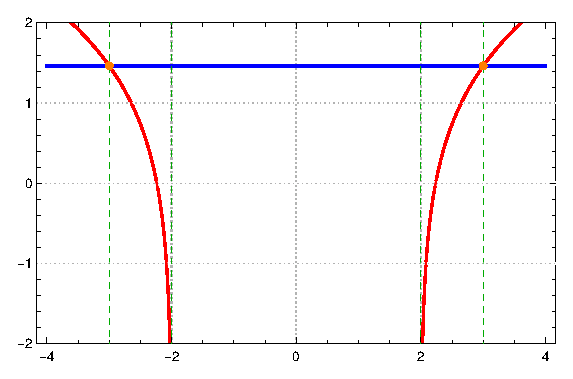
\includegraphics[width=\sirina]{eps/9.eps}}{$y={\color{red}\log_3(x^2-4)};\, {\color{blue}\log_3 5}$.}
$$
